
In the last two decades major progress has been achieved in improving the representation 
of clouds in General Circulation Models (GCMs, or Global Climte Models). 
Nevertheless, clouds (and also aerosols) are still being one of the largest uncertainties 
in estimating and interpreting the changes of Earth's energy budget \cite{IPCC2013}. 
One of the main problems is that many atmospheric processes cannot be resolved by current model resolutions, 
which operate on spatial scales ranging from a few kilometers to hundreds of kilometers. 
The small-scale processes related to clouds (e.g., cloud formation) 
are implemented by means of parameterizations that connect grid box mean variables to sub-grid processes.
Imperfect parameterization of clouds will of course have a significant impact on other projected variables 
and hence, on the modeled climate sensitivity. 
Thus, it is quite evident that cloud modeling needs to be carefully evaluated and improved 
for increasing our confidence in climate projections.
% Even though reasonable parameterizations are developed it remains challenging to balance the system regarding 
% simplicity, realism, computational stability, and efficiency.

One way to further enhance our understanding of cloud microphysical processes 
(particularly for ice- and mixed-phase clouds) is to use high-resolution models (cloud-resolving models, CRMs).
They are important tools for testing and improving the parameterizations of cloud-controlling processes,
such as cumulus convection, turbulent mixing, and aerosol-cloud interaction \cite{IPCC2013}.

The other possibility is to evaluate the simulation of clouds in GCMs by comparing
the model predictions with global satellite measurements.
However, it is not as simple as it sounds because there are significant differences
between cloud variables derived from models and satellite observations regarding
the spatial resolution, retrieval method, and definition.

Satellite retrievals use the measured intensity of radiation
from a particular area and direction at a particular wavelength and 
infer the cloud properties by solving the inverse problem.
This implies that several assumptions and auxiliary data are required in the forward modeling
causing limitations in deriving the geophysical quantity. For instance,
a retrieval might be sensitive to the first guess of the atmospheric state that is used in the inversion.
Moreover, passive space-borne instruments observe only the top of a cloud, while active sensors 
are able to resolve a cloud in the vertical direction but at the expense of a worse daily global coverage.
Consequently, it is plausible that a direct inter-comparison of simulated and observed clouds 
is not feasible without building a bridge that makes them comparable.

Cloud simulators are the answer to this problem. 
Figure~\ref{fig:sim_over} shows the general concept of how to bring model and observation land 
together in order to diagnose the cloud parameterization in modern climate models.
The key question to be answered is: 
``What would a satellite see if the atmosphere had the clouds of a climate model?'' 
Thus, the principle task of the simulator is to synthesize space-borne measurements of clouds 
from model states so that differences can be interpreted as model errors.
GCMs provide grid box mean profiles (e.g. cloud fraction, cloud water content, temperature, etc.)
and surface parameters (e.g. surface geopotential, land/sea mask, skin temperature, etc.),
which serve as input to the cloud simulator.
In general simulators consist of three modules:
\begin{enumerate}\setlength\itemsep{0.2em}
 \item Downscaler: It converts the grid box mean profiles into sub-grid profiles considering
 the mismatch in spatial scale between that of the model grid box ($\sim$ 100 km) and 
 that of a satellite pixel ($\sim$ 1 km). These subcolumns can be regarded as small samples that
 are assumed to be homogeneous, however, the large ensemble of them shall represent any 
 internal inhomogeneity in the grid cell.
 \item Pseudo-retrieval: It emulates the pixel-scale cloud parameters based on the sub-grid profiles
 and takes into account the retrieval characteristics of a particular algorithm.
 \item Statistical aggregation: It builds the diagnostic output that is comparable to the 
 observational dataset (i.e. temporal averages and joint histograms).
\end{enumerate}

The era of satellite simulators for evaluating climate model clouds began with the 
ISCCP (International Satellite Cloud Climatology Project) software package in 1999 \cite{Klein1999}.
The ISCCP dataset \cite{Rossow1999} along with its corresponding simulator have been used
in various studies that diagnosed the perfomance of GCMs. They have shown that common climate models
at that time underestimated the total cloud cover, overestimated optically thick clouds, and
underestimated midlevel clouds \cite{Kay2012}. 
Since then, many other simulators for cloud-related instruments \cite{Pincus2012} 
followed contributing to further improve cloud parameterizations in GCMs.\\
A widely used and state-of-the-art diagnostic tool is COSP (CFMIP Observation Simulator Package), 
which has been developed by the Cloud Feedback Model Intercomparison Project (CFMIP) community \cite{Bodas2011}.
COSP is capable to simulate observations of multiple active and passive satellite instruments
(e.g., CloudSat, Calipso, ISCCP, MISR, MODIS) and therefore, allows the quantitative evaluation of 
clouds, humidity, and precipitation processes in diverse numerical models.

In this study the ERA-Interim clouds are evaluated using a simulator that brings
the cloud properties mimicked by the forecast model and those provided by the 
ESA Cloud\_cci project based on AVHRR and MODIS observations on the same footing 
so that model deficiencies can be identified.
However, it is important to note that like all models, instrument simulators are incomplete
because it is not possible to include everything about the observational process 
(e.g. satellite view angle effects on cloud detection, 
artifacts caused by partially cloudy satellite pixels) in the simulator.
Hence, cloud simulators cannot entirely close the gap between models and observations of clouds,
but they are essential diagnostic tools when carrying out robust inter-comparisons
(e.g. excluding clouds with very low optical thickness).

The article is organized as follows. Section~\ref{sec:datasets} describes how clouds 
are parameterized in ERA-Interim and introduces the ESA Cloud\_cci project.
The cloud simulator developed for this study is explained in Section~\ref{sec:sim}.
The inter-comparison of pseudo-satellite and observed cloud parameters is given in Section~\ref{sec:sim_vs_obs}.
Finally, Section~\ref{sec:sum_and_con} closes with a summary and conclusions. 

\begin{figure}[!t]
 \centering
 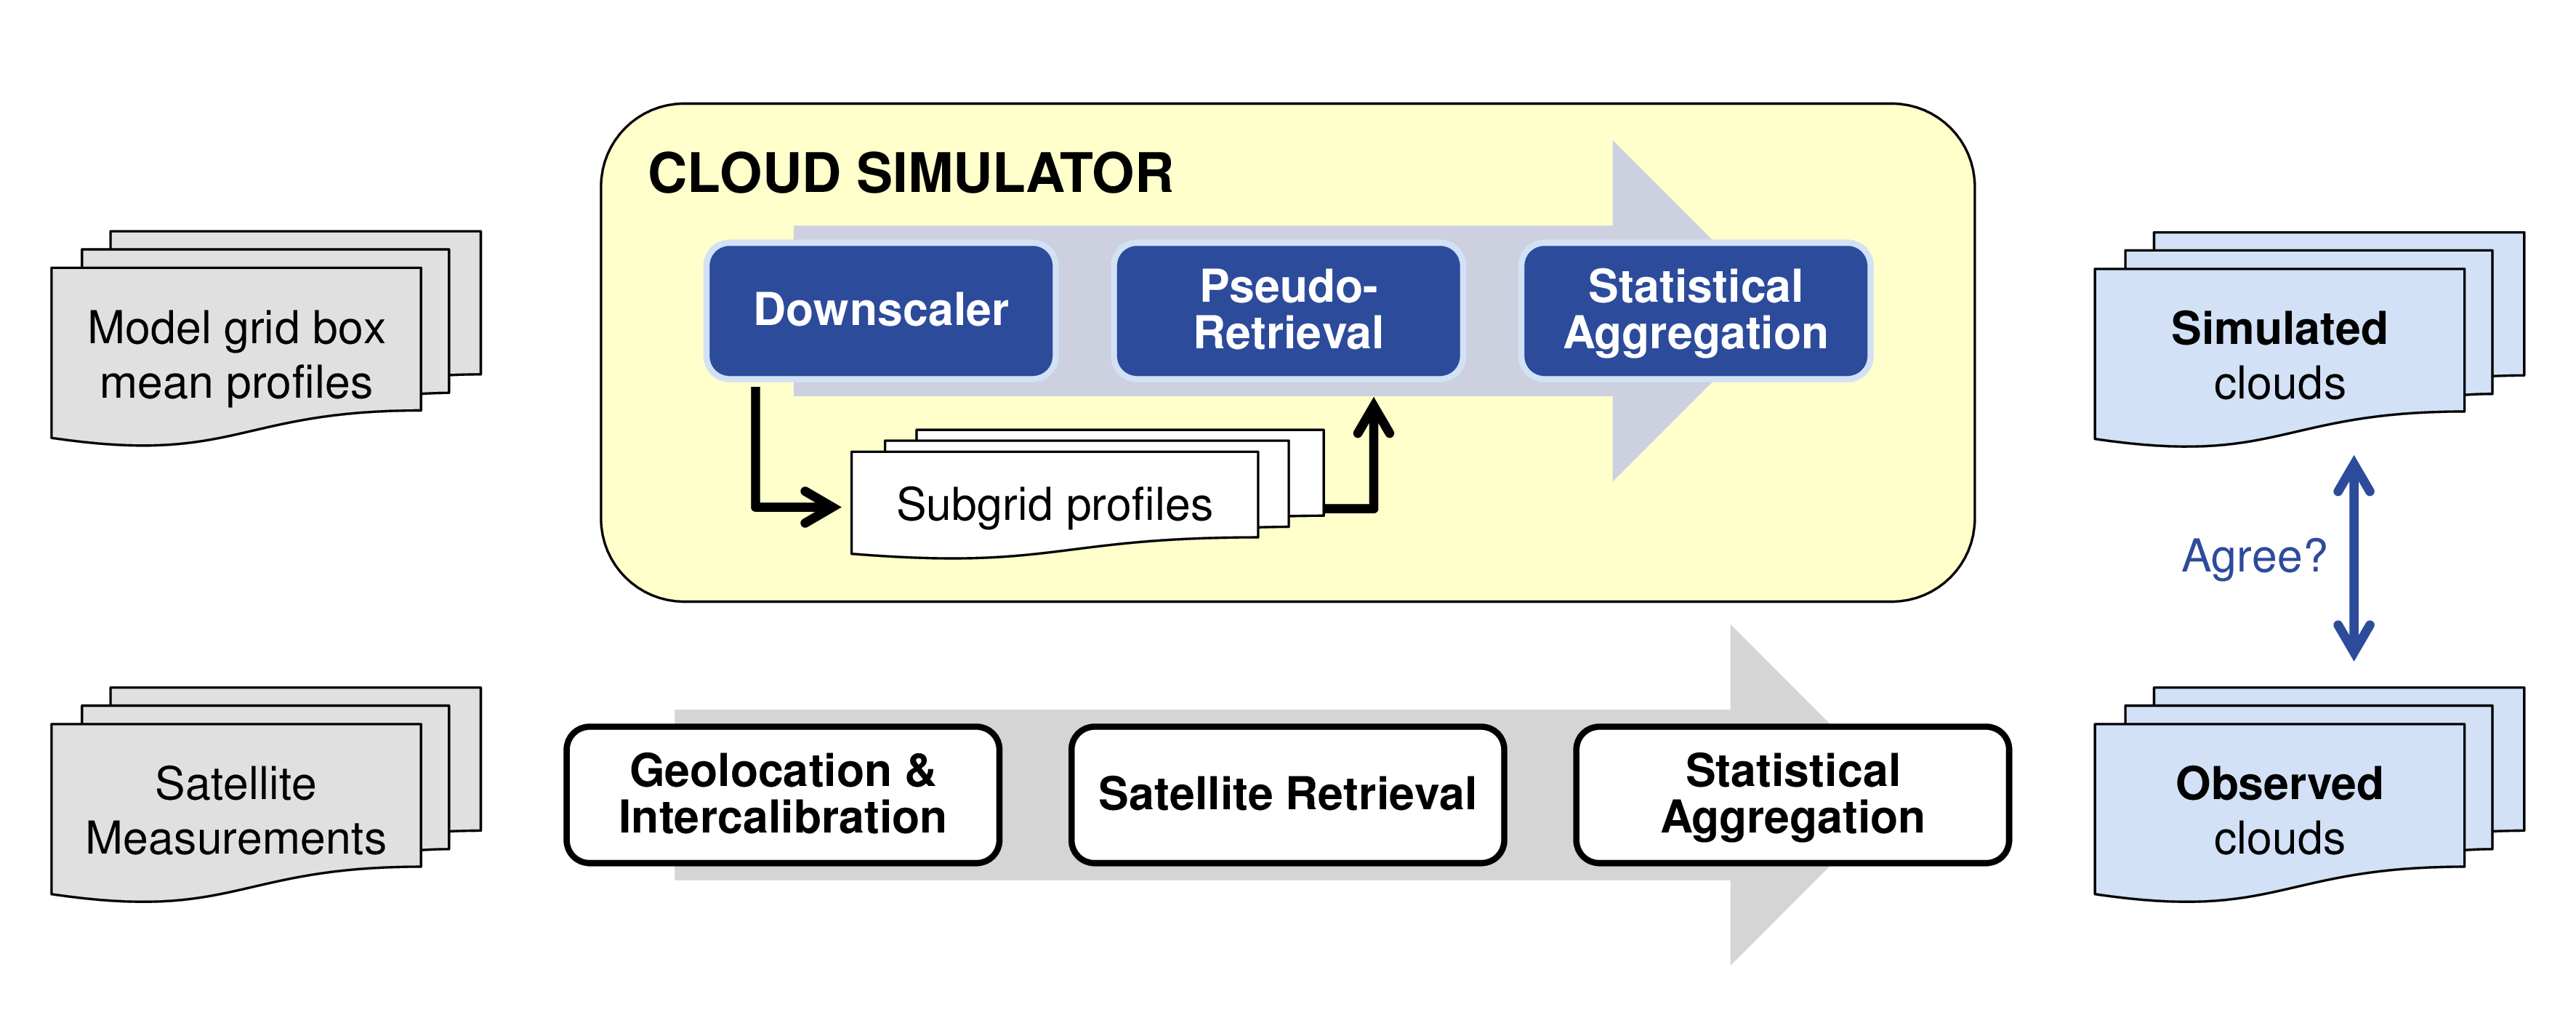
\includegraphics[width=\textwidth]{./figures/simulator_overview.png}
 \caption[Simulator evaluation concept.]
 {Schematic representation of how to use a clouds simulator to evaluate the
 cloud parameterization in global climate models. The simulator is a piece of 
 diagnostic code that maps the model representation to synthetic observations 
 with the objective of enabling the comparison between simulated and observed clouds.
 % making the simulated cloud variables comparable to the satellite-based products.
 It is accomplished by reproducing the internal description of clouds in a model 
 along with the retrieval characteristics of a particular algorithm and generating
 statistics that is comparable with the observational data record.}\label{fig:sim_over}
\end{figure}
